The explanations were computed for the selected equal-weight gate of seed 42 on 300 randomly drawn
validation (fold-9) records, which contain 131 NORM, 81 MI, 65 STTC, 80 CD and 31 HYP positives;
the test fold was not used. Fig.~\ref{fig:xaileads} shows the global lead importance, i.e.\ the share
of the absolute Integrated-Gradients attribution falling on each lead, averaged over the positive
records of each class. Under a uniform distribution every lead would receive 8.3\%.

\begin{figure}[!t]
\centering
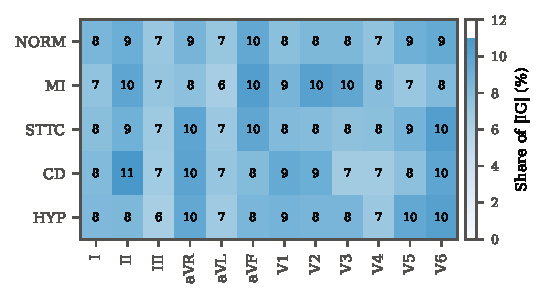
\includegraphics[width=\columnwidth]{xai_leads}
\caption{Global explanation: share of the absolute Integrated-Gradients attribution per lead (\%)
for the positive validation records of each superclass (seed 42, equal-weight gate).}
\label{fig:xaileads}
\end{figure}

The attributions are spread over all twelve leads (no lead receives more than 11.0\%), which is
consistent with the redundancy of the leads shown in Fig.~\ref{fig:leadcorr} and with training under
lead dropout. Within this spread the emphasis follows the expected anatomy. For MI the largest shares
fall on aVF (10.3\%), V2 (10.1\%), II (9.8\%) and V3 (9.7\%), i.e.\ on the inferior and anteroseptal
leads that record the most frequent infarct locations. For HYP the largest shares fall on V6
(10.3\%), V5 and aVR (9.6\% each) and V1 (8.6\%), the leads used by the classical voltage criteria
for left ventricular hypertrophy, which combine the S wave in V1 with the R wave in V5 or V6. For CD
the model relies most on II (11.0\%), aVR (9.9\%), V6 (9.8\%) and V1 (9.4\%); V1 and V6 are the leads
in which right and left bundle branch blocks are recognised. STTC is attributed mainly to the
lateral and inferior leads V6 (10.3\%), aVR (9.8\%) and aVF (9.7\%). In every class, leads III and aVL
are among the four least-attributed leads (6.2\%--7.2\%); both are linear combinations of I and II,
so they add little independent information.

\textit{Local explanations.} Fig.~\ref{fig:xailocal} shows the two validation records predicted with
the highest confidence for MI and for STTC, with the three leads that carry the largest attribution
and the attribution magnitude along time. Record 5927 (label MI) is classified as MI with probability
0.99, and its attribution concentrates on V2, V3 and V4. These leads show deep, predominantly negative
QRS complexes, the pattern of an anterior infarction, and the attribution peaks at each QRS complex
rather than in the baseline between beats. Record 14758 (labels STTC and HYP) receives P(STTC) = 0.98
and P(HYP) = 0.85, so both of its labels are recovered; for STTC the attribution falls on V2, V1 and
aVF and again peaks at the QRS complexes and the adjoining ST segments of the beats. In both cases the
attribution is locked to the beats and falls on the waveform segments a cardiologist would inspect,
not on the baseline between beats; two examples cannot, however, establish this for all records.

\begin{figure*}[!t]
\centering
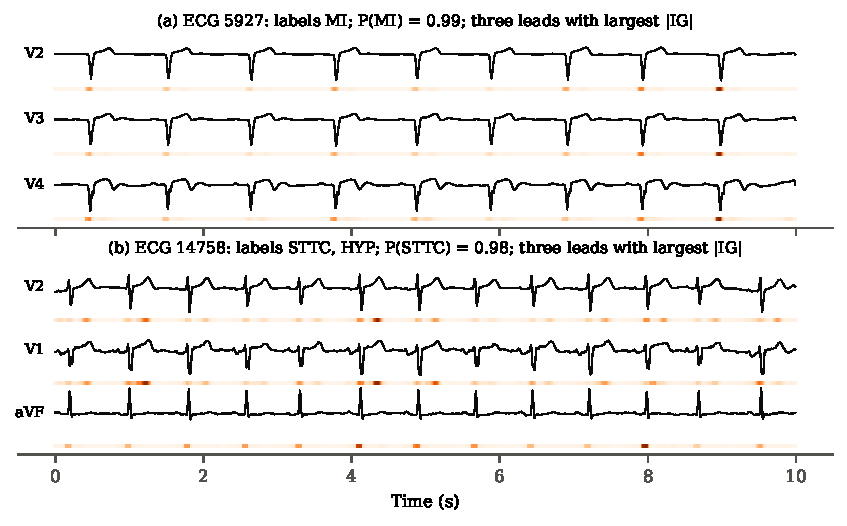
\includegraphics[width=0.95\textwidth]{xai_local}
\caption{Local explanations for the most confident true-positive (a) MI and (b) STTC validation
records. For each record the three leads with the largest total attribution are shown; the colour
strip below each trace encodes $|\mathrm{IG}|$ over time (darker = larger), smoothed over 90~ms.}
\label{fig:xailocal}
\end{figure*}

\textit{Faithfulness.} Table~\ref{tab:deletion} reports the deletion test. For NORM, MI and CD,
removing the lead with the largest attribution lowers the mean predicted probability more than
removing a random lead (NORM: $-$0.028 versus $-$0.019; MI: $-$0.030 versus $-$0.006; CD: $-$0.043
versus $-$0.012), and removing the three most important leads lowers it substantially more than
removing three random leads (NORM: $-$0.135 versus $-$0.074; MI: $-$0.057 versus $-$0.006; CD:
$-$0.070 versus $-$0.009). For these classes the attributions therefore identify leads on which the
prediction actually depends. For STTC and HYP, in contrast, neither targeted nor random deletion
changes the probability appreciably (STTC: 0.764 intact, 0.765--0.772 after deletion; HYP: 0.620
intact, 0.613--0.627 after deletion). The evidence for these two classes is distributed redundantly
over many leads, so lead-level attributions should not be read as identifying a single decisive lead.

\begin{table}[!t]
\centering
\caption{Deletion test: mean gate probability of the true class after zeroing the $k$ leads with the
largest IG attribution or $k$ random leads (fold-9 positives, seed 42)}
\label{tab:deletion}
\footnotesize
\setlength{\tabcolsep}{4pt}
\resizebox{\columnwidth}{!}{\begin{tabular}{@{}lcccccc@{}}
\toprule
 & & & \multicolumn{2}{c}{Top-$k$ IG leads removed} & \multicolumn{2}{c}{Random $k$ leads removed} \\
\cmidrule(lr){4-5}\cmidrule(l){6-7}
Class & $n$ & Mean $p$ (intact) & $k=1$ & $k=3$ & $k=1$ & $k=3$ \\
\midrule
NORM & 131 & 0.741 & 0.713 & 0.606 & 0.722 & 0.667 \\
MI & 81 & 0.750 & 0.720 & 0.693 & 0.744 & 0.744 \\
STTC & 65 & 0.764 & 0.765 & 0.772 & 0.764 & 0.771 \\
CD & 80 & 0.758 & 0.715 & 0.688 & 0.746 & 0.749 \\
HYP & 31 & 0.620 & 0.626 & 0.621 & 0.627 & 0.613 \\
\bottomrule
\end{tabular}
}
\end{table}

\textit{Federation-level explanation.} At the level of the institutions, the Shapley values in
Table~\ref{tab:shapley} show that the four clients contribute comparably to the AUROC of the
federation (0.097--0.105 on the test fold), with the recurrent clients C and D contributing most.
Together with the signal-level attributions, this gives a clinician two complementary views: which
leads and waveform segments drove a finding, and which participating sites the global model relied on.
These explanations are post hoc and were not yet reviewed by cardiologists, and IG with a zero
baseline, like every attribution method, depends on the choice of baseline.
